%*******************************************************************************
%                                                                              *
%                 Datei: header.tex                                            *
%                                                                              *
%                 Stand: 10.10.2013   11.02 Uhr   (Elt)                        *
%                                                                              *
%*******************************************************************************

\documentclass[%
    paper=a4,            % Layout fuer Din A4
    %oneside,          % einseitiger Druck
	twoside,             % Layout fuer beidseitigen Druck
    fontsize=12pt,       % Schriftgroesse 12pt
    %openright,        % Kapitel dürfen nur auf einer rechten Seite beginnen
    openany,          % Kapitel dürfen rechts oder links beginnen
    halfparskip,      % eine halbe Zeile Abstand zw. Absätzen
    headsepline,         % horizontale Linie unter Kolumnentitel
    headinclude,         % Kopfzeile wird Seiten-Layouts mit beruecksichtigt
    plainheadsepline,    % horizontale Linie auch beim plain-Style
    %footsepline,      % Fußzeilenlinie
    parskip=half,        % Absatzabstand statt Absatzeinzu
    bibliography=totoc,  % Literaturverz. wird ins Inhaltsverzeichnis eingetragen
    %idxtotoc,          % Index im Inhaltsverzeichnis
    listof=totoc,        % Abbildungs und TabellenVZ ins InhaltsVZ
    ]{scrbook}


\usepackage{longtable}
\usepackage{titlesec}% Ändert die Größe der Überschriften subsubsection
%\titleformat*{\subsubsection}{\large\bfseries}

\usepackage[utf8]{inputenc}
\usepackage{titleref}
% deutsche Silbentrennung etc.
\usepackage[ngerman]{babel}      % neue Rechtschreibung

%schriftarten
\usepackage[T1]{fontenc}
\newcommand{\changefont}[3]{
\fontfamily{#1} \fontseries{#2} \fontshape{#3} \selectfont}

%abkürzungsverzeichnis
\usepackage[printonlyused, footnote, nohyperlinks]{acronym}
%\usepackage{glossaries}

%\usepackage{natbib}
\usepackage[square,sort,comma,numbers]{natbib}

%fußnote nummerierung durchgehen
\usepackage{chngcntr} 
\counterwithout{footnote}{chapter}

% Grafiken: PDF, GIF, PNG
\usepackage{graphicx}
\usepackage{subfigure}
\usepackage{pdfpages}
\usepackage{float}
\usepackage{wrapfig}


%tür tabellen
%\usepackage{booktabs}

% Farben
\usepackage{color}
\definecolor{link_color}{rgb}{0,0,0.6}
\definecolor{ListingBG}{rgb}{0.95,0.95,0.95}

% Hyperlinks (anklickbar im PDF)
\usepackage[%
    pdftitle={Sortieralgorithmus Bubblesort},%
    pdfauthor={Nick Koslowski},%
    pdfpagemode=UseOutlines
]{hyperref}   

\usepackage{blindtext}
    
\hypersetup {
     breaklinks = {true},      % Erlaubt Zeilenumbrüche in Links
     colorlinks = {true},      % Benutze farbige Links
     citecolor = {link_color}, % Farbe für Zitate
     linkcolor = {link_color}, % beeinflusst Inhaltsverz. und Seitenzahlen
     urlcolor = {link_color},  % Weblink-Farbe
     pdftitle = {Sortieralgorithmus Bubblesort}, % Titel der Arbeit
     pdfsubject = {Unterweisungsentwurf}, % Thema der Arbeit
     pdfauthor = {Nick Koslowski},  % AutorIN der Arbeit
     pdfkeywords = {Hier ein paar Stichwörter}, % Stichwörter zur Arbeit
     pdfproducer = {pdfLaTeX}, % Erzeugt durch
     pdfcreator = {MacTeX},    % Erstellt mit
     pdfstartview = {FitV},
     pdfview = {FitH},
     pdffitwindow = {true}
}


% Quellcode Formatierung
\usepackage{listings}
\lstset{%
    language=Python, % Programmiersprache
    numbers=left, % Zeilennummern
    stepnumber=1, % jede Zeile
    numbersep=5pt, % Abstand zum Quellcode
    numberstyle=\tiny, % Schriftgröße
    breaklines=true, % Zeilenumbrüche zulassen
    breakautoindent=true, % Einrücken nach Umbruch
    tabsize=2,  % Tabulator
    basicstyle=\footnotesize, %
    showspaces=false, % Leerzeichen anzeigen (true -> underscore)
    showstringspaces=false, % Leerzeichen in Strings
    backgroundcolor=\color{ListingBG}, % Hintergrundfarbe
    captionpos=b,   % Position der Beschreibung (b: bottom)
    %keywordstyle=\color{red}\bfseries
}

\usepackage{setspace}       % Zeilenabstand einstellbar
\onehalfspacing             % eineinhalbzeilig einstellen
\usepackage{scrpage2}       % Kopf und Fusszeilen-Layout 


\renewcommand{\headfont}{\normalfont\sffamily}    % Kolumnentitel serifenlos
\renewcommand{\pnumfont}{\normalfont\sffamily}    % Seitennummern serifenlos
\pagestyle{scrheadings}
\ihead[]{\headmark}              % Kolumnentitel immer oben innen
\ohead[\pagemark]{\pagemark}     % Seitennummern immer oben aussen
\ofoot[]{}                       % Seitennummern in der Fusszeile loeschen

\renewcommand{\bibname}{Literatur} % Literaturverzeichnis wird zu Literatur
\renewcommand{\figurename}{Abb.}   % Abbildung wird zu Bild

% erweiterte Tabellen
\usepackage{array}

% Formelsatz
\usepackage{amsmath}

% Definition eigener Operatoren (im Header)
\DeclareMathOperator{\rg}{Rang}  

% Fortlaufende Kapitelüberschriften in der Kopfzeile
%\pagestyle{headings}

% Stil des Literaturverzeichnis
\bibliographystyle{alphadin}

%text im Literaturverzeichnis
\setbibpreamble{Auflistung aller Quellen, die zum erstellen dieses Dokumentes verwendet wurden.\par\bigskip}

\begin{document}
\begin{titlepage}
\center
Unterweisungsentwurf zur Ausbilder-Eignungsprüfung\\[1.5cm]



\parbox{0.85\textwidth}{
\begin{center}
{\huge \bfseries Sortieralgorithmus \\[0.5cm] Bubblesort }
%Anschauliche Darstellung \\ eines Algorithmus am \\ Beispiel von Bubblesort \\ 
\end{center}
}
\\[1cm]


\begin{figure}[H]
\centering

\includegraphics[scale=0.25]{bubblesort}
\end{figure}

{\bfseries Fachinformatiker \\}
(Fachrichtung Anwendungsentwickung)

\vfill
\today \\[0.5cm]
\copyright \xspace Nick Koslowski


\end{titlepage}

\frontmatter
\pagenumbering{Roman}
\chapter{Angaben zur Person}
{
\begin{tabular}{p{3.06cm}cl}
Name &:& Nick Koslowski\\[0.5ex]
Alter &:& \\[0.5ex]
Anschrift &:& \\[0.5ex]
Arbeitgeber &:& \\[0.5ex]
\end{tabular}
}

{
\let\clearpage\relax 
\chapter{Angaben zur Prüfung}
\begin{tabular}{p{3.06cm}cl}
Prüflingsnummer &:& \\[0.5ex]
Zuständige Stelle &:& IHK Braunschweig\\[0.5ex]
Prüftermin &:& 15.11.2023\\[0.5ex]
Thema &:& Sortieralgorithmus Bubblesort\\[0.5ex]
\end{tabular}
}

\chapter*{Erklärung}
\addcontentsline{toc}{chapter}{Erklärung}
\thispagestyle{empty}

   \vspace*{2,5cm}
Hiermit versichere ich, dass ich den vorliegenden Unterweisungsentwurf zur Ausbilder-Eignungsprüfung selbständig nur unter Zuhilfenahme der ausgewiesenen Hilfsmittel angefertigt habe.
   \vspace*{3em}\\
     Braunschweig, \today \hfill \parbox[t]{5cm}{\centering\hrule\medskip Nick Koslowski}


\cleardoubleemptypage
%\listoffigures
%\cleardoubleemptypage
%\listoftables
%\cleardoubleemptypage
%\lstlistoflistings 
%\cleardoubleemptypage
\tableofcontents

\mainmatter

\chapter{Didaktische Analyse}
{
\begin{tabular}{p{2.8cm}cl}
Ausbildungsberuf &:& Fachinformatiker\\[0.5ex]
&& Fachrichtung Anwendungsentwicklung\\[0.5ex]
Ausbildungsjahr &:& 2. Ausbildungsjahr\\[0.5ex]
\end{tabular}
}

\section{Thema der Unterweisung}

Fachinformatiker der Fachrichtung Anwendungsentwicklung verbringen einen Großteil ihrer Zeit mit der Entwicklung und Optimierung von Softwareanwendungen. Dabei bilden Algorithmen die Grundlage für das Programmieren, indem komplexe Aufgaben in klar definierte Schritte zerlegt und so gelöst werden. Um den Auszubildenden Algorithmen näher zu bringen und in die Lage zu versetzen, das schrittweise Vorgehen eines Algorithmus zu verstehen, wird den Auszubildenden der Sortieralgorithmus Bubblesort anschaulich vermittelt. Die Auszubildenden sollen den Bubblesort verstehen und anwenden können.


\chapter{Lernzielbeschreibung}
Im folgenden Abschnitt werden die konkreten Ziele der Unterweisung aufgeführt.

\section{Richtlernziel}
Das Richtlernziel ist das Entwickeln, Erstellen und Betreuen von IT-Lösungen (§ 4 Absatz 2 Nummer 4).

\section{Groblernziel}
Die Auszubildenden sollen Algorithmen durchführen und formulieren können (Nummer 4 Abschnitt b).

\section{Feinlernziel}
Die Auszubildenden sind nach dieser Unterweisung in der Lage, die Funktionsweise des Bubblesort-Algorithmus mit eigenen Worten zu beschreiben und diesen anzuwenden.

\chapter{Lernbereiche}
\section{Kognitiver Lernbereich}

%Die Auszubildenden lernen das algorithmische Vorgehen zum Lösen komplexer Aufgaben, indem sie durch das Durchführen klar definierter Schritte unter Einhaltung der korrekten Reihenfolge zur Lösung gelangen. Darüber hinaus lernen sie anhand festgelegter Kriterien Elemente zu vergleichen, den Vergleich zu bewerten sowie die entsprechende Handlung daraus abzuleiten.

In dieser Unterweisung lernen die Auszubildenden die einzelnen Teilschritte des Bubblesort-Algorithmus kennen und wissen, wie und in welcher Reihenfolge diese anzuwenden sind. Darüber hinaus wird die Abstraktionsfähigkeit zur Lösung komplexer Probleme durch das Herunterbrechen in kleine Teilschritte geschärft.

\section{Affektiver Lernbereich}

Den Auszubildenden wird die Wichtigkeit der genauen und definierten Durchführung von Arbeitsschritten vermittelt, um unter denselben Bedingungen immer zum selben Ergebnis zu gelangen. Damit wird die Sorgfaltspflicht der Auszubildenden geschult. Des Weiteren wird durch die spielerische Darstellung das Interesse sowie die Motivation zur Lernbereitschaft gefördert. 


%\section{Psychomotorischer Lernbereich}
%Auszubildende lernen die praktischen Fähigkeiten Eingaben damit schulen die Psychomotorischen

%\chapter{Schlüsselqualifikationen}

%\begin{itemize}
%\item Teamfähigkeit
%\item Kommunikationsfähigkeit
%\item Selbstständigkeit
%\end{itemize}

\chapter{Ablauf der Unterweisung}

\section{Unterweisungsmethode}
In Stufe eins erfolgt bereits die Demonstration.

Für die Unterweisung wird eine abgewandelte Form der Vier-Stufen-Methode angewendet. Hierbei erfolgt bereits in der ersten Stufe die Demonstration des noch Unbekannten, um die Neugierde zu wecken. Daraus folgend werden die Arbeitsschritte in der zweiten Stufe den Auszubildenden nicht erläutert, sondern basierend auf der vorherigen Demonstration mit den Auszubildenden in einer geleiteten Diskussion erarbeitet und von ihnen selbstständig in die richtige Reihenfolge gebracht. In der dritten Stufe folgt zunächst die Überprüfung der Reihenfolge, bevor die Auszubildenden den erarbeiteten Algorithmus selbstständig durchführen. Die Kontrolle der korrekten Ausführung erfolgt durch die Betrachtung der Ergebnisse. In der vierten Phase erfolgt die Lernerfolgssicherung durch die eigenständige Wiedergabe der Arbeitsschritte durch die Auszubildenden.

\section{Ablaufplan}

Im Folgenden wird der geplante Ablauf der Unterweisung beschrieben und aufgezeigt.

\pagebreak
\subsection{Unterweisungsstufen}
\begin{longtable}{ |p{3cm}|p{3cm}|p{3cm}|p{3cm}|}
\hline
\textbf{Was} & \textbf{Wie} & \textbf{Warum} & \textbf{Hilfsmittel} \\
\hline
\multicolumn{4}{|l|}{\textbf{Stufe 1: Vorbereitung}}  \\
 \hline
Begrüßung  & Schaffung einer angenehmen Atmosphäre  & Entspannung und Abbau von Hemmungen & \\
 \hline
 Vorkenntnisse \& Thema der Unterweisung & Demonstration des Algorithmus mit Spielkarten, Benennung des Unterweisungsthemas und gezieltes Erfragen der Vorkenntnisse & Spielerisches Heranführen an das Unterweisungsthema und Prüfen bereits vorhandener Kenntnisse & Spielkarten\\
 \hline
Lernziel  & Thema und Fragestellung an das Whiteboard anbringen & Benennung des Feinlernziels & Vorbereitete Zettel \& Magnete  \\
 \hline
  \pagebreak
   \hline
  \textbf{Was} & \textbf{Wie} & \textbf{Warum} & \textbf{Hilfsmittel} \\
 \hline
\multicolumn{4}{|l|}{\textbf{Stufe 2: Lehrgespräch und Erarbeitung der Schritte}}  \\
\hline
 Geleitete Diskussion & Durch Nachfragen des Gesehenen in der Demonstration & Zur Aktivierung der Auszubildenden und Reflexion des Gesehenen & \\
 \hline
 Begriffserläute- rung & Erklären was unter dem Begriff Algorithmus zu verstehen ist & Zur Schaffung eines besseren Verständnisses & \\
 \hline
Erarbeitung der Schrittreihenfolge  & Den Auszubildenden werden die Teilschritte des Algorithmus ausgehändigt mit dem Auftrag, diese selbstständig in die richtige Reihenfolge zu bringen & Zur Erarbeitung des Algorithmus sowie der Förderung der Zusammenarbeit  & Vorbereitete Zettel mit den Teilschritten \& Pinnwandnadeln\\
 \hline
\multicolumn{4}{|l|}{\textbf{Stufe 3: Durchführung und Selbstkontrolle}}  \\
\hline
Kontrolle der Reihenfolge der Schritte & Der Ausbilder überprüft die Korrektheit der  Schrittreihenfolge & Zur Sicherstellung der Voraussetzungen zur korrekten Durchführung  & \\
 \hline
Nachmachen  & Die Anwendung des Algorithmus mit verdeckten Spielkarten & Verfestigung der Teilschritte & Spielkarten\\
 \hline
 \pagebreak
  \hline
   \textbf{Was} & \textbf{Wie} & \textbf{Warum} & \textbf{Hilfsmittel} \\
 \hline
Kontrolle des Ergebnisses  & Die Auszubildenden prüfen durch das Umdrehen der Spielkarten selbstständig das Sortierergebnis & Auszubildende erkennen, ob der Algorithmus korrekt durchgeführt wurde & Spielkarten \\
 \hline
\multicolumn{4}{|l|}{\textbf{Stufe 4: Lernerfolgssicherung und Bewertung}}  \\
\hline
Lernerfolgs- kontrolle & Überprüfung der Schritte mit eigenen Worten  & Zur Messung des Lernerfolgs & \\
 \hline
Bewertung & Wissenswieder- gabe beurteilen und bei Bedarf korrigieren & Feedback zur erbrachten Leistung & \\
 \hline
Abschluss \& Verabschiedung  &  Auszubildende werden freundlich verabschiedet & Wertschätzung für Mitarbeit & \\
\hline
\end{longtable}

.

\appendix       %Beginn des Anhangs

\chapter{Anhang}
\begin{figure}[H]
\centering
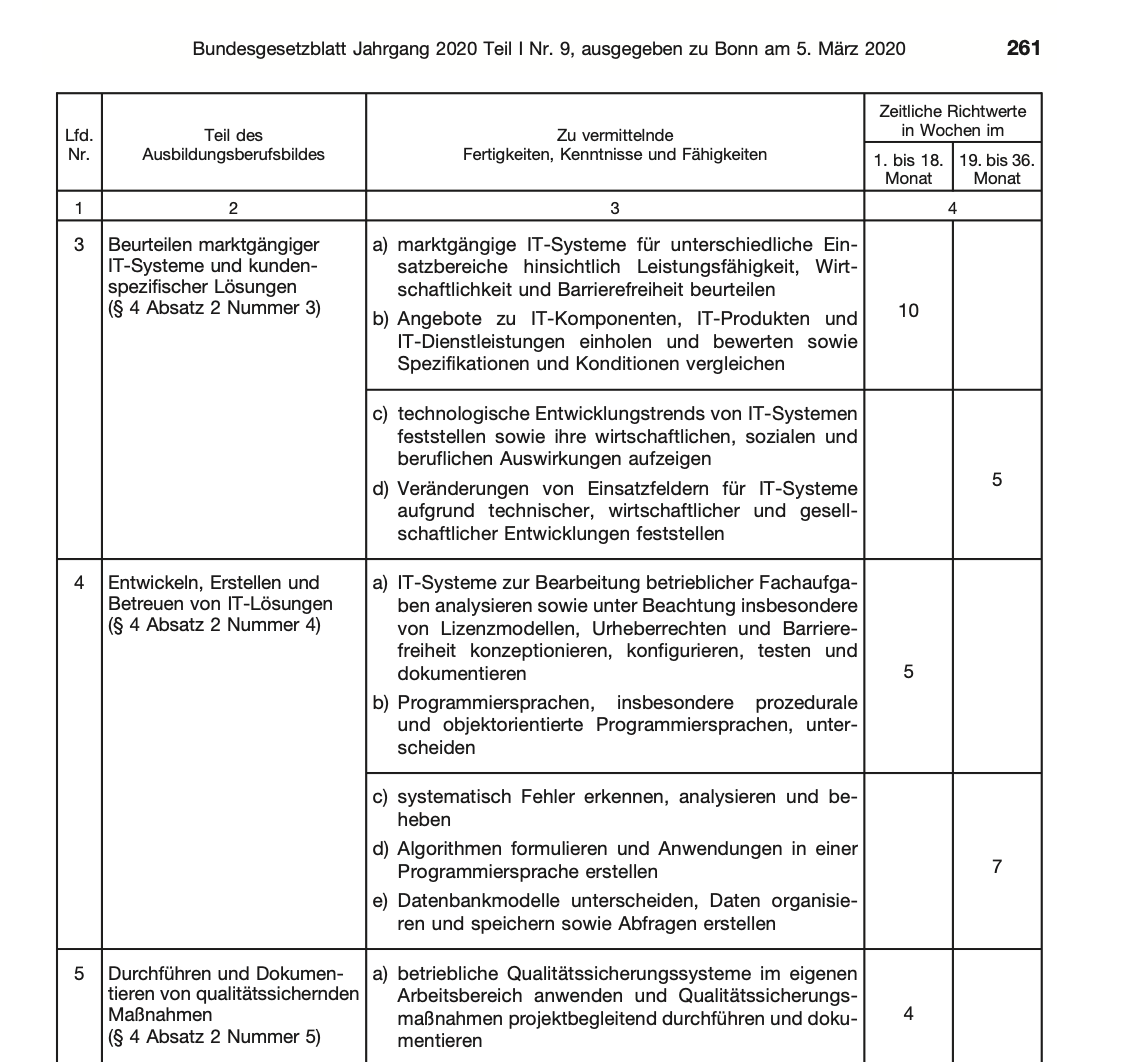
\includegraphics[scale=0.9]{arp}
\caption{Auszug aus der Fachinformatikerausbildungsverordnung}
\end{figure}




\end{document}
